\section{Fisher线性判别分析}
\subsection{二类线性判别法}
(Fisher)线性判别分析(Linear Discriminant Analysis,简称FDA)是一种经典的线性学习算法。思想是:给定训练样例集,设法将样例投影到一条直线上,使得同类样例的投影点尽量接近,不同类的投影点尽可能远。对于要预测的数据点,投影之后,按位置来划分样本类别。
\begin{center}
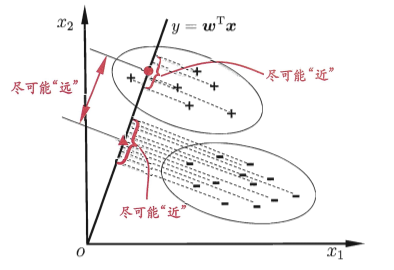
\includegraphics[scale=1]{../figures/LDA1.PNG} 
\end{center}
对于二分类问题,给定数据集$D=\{\sample{x}{i},\sample{y}{i}\}^m_{i=1},y_i\in \{0,1\}$,令$X_i,\mu_i,S_i$分别表示第$i\in\{0,1\}$类的样本的集合、均值向量、协方差矩阵。
\begin{eqnarray}
\mu_i &=& \frac{1}{N_i}\sum_{j\in C_i}\sample{x}{j} = \frac{1}{N_i}\sum_{j=1}^N \sample{x}{j}1(\sample{y}{j}=i)\\
S_i &=& \sum_{j\in C_i}(\sample{x}{j}-\mu_i)(\sample{x}{j}-\mu_i)^T = \sum_{j=1}^N (\sample{x}{j}-\mu_i)(\sample{x}{j}-\mu_i)^T1(\sample{y}{j}=i)
\end{eqnarray}
其中,$C_i$代表第$i\in\{0,1\}$类的样本的集合,$N_i$代表第$i\in\{0,1\}$类的样本个数,$N=N_1+N_2$,$1()$代表示性函数。

若将数据投影到向量$w$(列向量),即$w^Tx$,则第$i$类的均指向量在$w$上的投影为
\begin{eqnarray}
\begin{aligned}
&\ \frac{1}{N_i}\sum_{j\in C_i}w^T\sample{x}{j}\\
&=w^T\frac{1}{N_i}\sum_{j\in C_i}\sample{x}{j}\\
&=w^T\mu_i
\end{aligned}
\end{eqnarray}
第$i$类的协方差在$w$上的投影为
\begin{eqnarray}
\begin{aligned}
&\ \sum_{j\in C_i}(w^T\sample{x}{j}-w^T\mu_i)(w^T\sample{x}{j}-\mu_i)^T\\
&=\sum_{j\in C_i}(w^T(\sample{x}{j}-\mu_i))(w^T(\sample{x}{j}-\mu_i))^T\\
&=\sum_{j\in C_i}w^T(\sample{x}{j}-\mu_i)(\sample{x}{j}-\mu_i)^Tw\\
&=w^T\sum_{j\in C_i}(\sample{x}{j}-\mu_i)(\sample{x}{j}-\mu_i)^Tw\\
&=w^TS_iw
\end{aligned}
\end{eqnarray}
所以$w^T\mu_i$和$w^TS_iw$均为实数。

让类中心距离尽可能大,即$||w^T\mu_0-w^T\mu_1||^2_2$尽可能大,让同类样例投影点协方差尽可能小,即$w^TS_0w+w^TS_1w$尽可能小,则可得到最大化的目标
\begin{eqnarray}
\begin{aligned}
J&=\frac{||w^T\mu_0-w^T\mu_1||^2_2}{w^TS_0w+w^TS_1w}\\
&=\frac{w^T(\mu_0-\mu_1)(\mu_0-\mu_1)^Tw}{w^T(S_0+S_1)w}
\end{aligned}
\end{eqnarray}
定义“类内三度矩阵”(within-class scatter matrix)
\begin{eqnarray}
\begin{aligned}
S_w &=S_0+S_1\\
&=\sum_{i\in C_0}(\sample{x}{i}-\mu_0)(\sample{x}{i}-\mu_0)^T+\sum_{i\in C_1}(\sample{x}{i}-\mu_1)(\sample{x}{i}-\mu_1)^T
\end{aligned}
\end{eqnarray}
定义“类间散度矩阵”(between-class scatter matrix)
\begin{eqnarray}
\begin{aligned}
S_b=(\mu_0-\mu_1)(\mu_0-\mu_1)^T
\end{aligned}
\end{eqnarray}
则有
\begin{eqnarray}
J=\frac{w^TS_bw}{w^TS_ww}
\end{eqnarray}
这是LDA的最大化目标,称为$S_b$与$S_w$的“广义瑞利商”(generalized Rayleigh quotient)。由于分子和分母都是关于$w$的二次项,因此解与$w$的长度无关,只与方向有关。不是一般性,令$w^TS_ww=1$,有
\begin{eqnarray}
\begin{aligned}
&\min_w\ -w^TS_bw\\
&s.t.\ w^TS_ww=1
\end{aligned}
\end{eqnarray}
使用拉格朗日乘子法,有
\begin{eqnarray}
L(w,\lambda)=-w^TS_bw+\lambda(w^TS_ww-1)
\end{eqnarray}
对$w,\lambda$求偏导,有
\begin{eqnarray}
\frac{\partial F}{\partial w}&=&-(S_b+S_b^T)w+\lambda(S_w+S_w^T)w=0\\
\frac{\partial F}{\partial \lambda}&=&1-w^TS_ww=0
\end{eqnarray}
得到
\begin{eqnarray}
S_bw&=&\lambda S_ww\\
w^TS_ww&=&1
\end{eqnarray}
由于$(\mu_0-\mu_1)^Tw$为常数,记$k=(\mu_0-\mu_1)^Tw$,则有
\begin{eqnarray}
S_bw=k(\mu_0-\mu_1)=\lambda S_ww
\end{eqnarray}
可得
\begin{eqnarray}
w=S_w^{-1}\frac{k}{\lambda}(\mu_0-\mu_1)
\end{eqnarray}
由于只需要得到$w$的方向,因而令$\frac{k}{\lambda}=1$,有
\begin{eqnarray}
w=S_w^{-1}(\mu_0-\mu_1)
\end{eqnarray}
对于$S_w^{-1}$的计算,为了数值解的稳定性,通常对$S_w$进行奇异值分解,有
$S_w=U\SigmaV^T$,之后有$S_w^{-1}=V\Sigma^{-1}U^T$。

对于一个新的数据点$x$,计算其投影点分别到$w^T\mu_1$和$w^T\mu_2$的距离,作差,有
\begin{eqnarray}
\begin{aligned}
D&=(w^T\mu_1-w^Tx)^2-(w^T\mu_2-w^Tx)^2\\
&=(w^T\mu_1)^2+(w^Tx)^2-2w^T\mu_1w^Tx-(w^T\mu_2)^2-(w^Tx)^2+2w^T\mu_2w^Tx\\
&=(w^T\mu_1)^2-(w^T\mu_2)^2-2(w^T\mu_1-w^T\mu_2)w^Tx\\
&=(w^T\mu_1+w^T\mu_2)(w^T\mu_1-w^T\mu_2)-2(w^T\mu_1-w^T\mu_2)w^Tx\\
&=(w^T\mu_1-w^T\mu_2)(w^T\mu_1+w^T\mu_2-2w^Tx)\\
&=(w^T\mu_1-w^T\mu_2)(w^T(\mu_1+\mu_2-2x))
\end{aligned}
\end{eqnarray}
当$w^T(\mu_1+\mu_2-2x)>0$时,$D>0$,则$x$判定为第2类;当$w^T(\mu_1+\mu_2-2x)<0$时,$D<0$,则$x$判定为第1类。